% Created 2021-11-03 mié 11:39
% Intended LaTeX compiler: lualatex
\documentclass[table]{scrartcl}
\usepackage[left=1.5cm,right=1.5cm,bottom=2.5cm,letterpaper]{geometry}
\usepackage[spanish, es-nodecimaldot, es-tabla]{babel}
\usepackage[utf8]{inputenc}
\usepackage{blindtext}
\usepackage{multicol}
\usepackage{subfigure}
\usepackage[most]{tcolorbox}
\usepackage{etoolbox}
\usepackage{minted}
\usepackage{hyperref}
% \usepackage[table,xcdraw]{xcolor}
\usepackage{longtable}

\usepackage[default]{comfortaa}
\usepackage[T1]{fontenc}

\usepackage{caption}
\usepackage{breqn}
\usemintedstyle{emacs}
\usepackage[ruled,vlined]{algorithm2e}
\newenvironment{code}{\captionsetup{type=listing}}{}
\definecolor{custom}{HTML}{F8F8F8}
\setminted{frame=lines,breaklines=true,bgcolor=custom,fontsize=\scriptsize,linenos}
\renewcommand{\listingscaption}{Código}
\renewcommand\listoflistingscaption{Índice de \listingscaption\@s}
\BeforeBeginEnvironment{listing}{\begin{code}}
  \AfterEndEnvironment{listing}{\end{code}}
\BeforeBeginEnvironment{minted}{\begin{code}}
  \AfterEndEnvironment{minted}{\end{code}}
\author{Monsalvo Bolaños Melissa Monserrat y Romero Andrade Cristian}
\date{\today}
\title{Practica 3}
\hypersetup{
  pdfauthor={Monsalvo Bolaños Melissa Monserrat y Romero Andrade Cristian},
  pdftitle={Practica 3},
  pdfkeywords={},
  pdfsubject={},
  pdfcreator={Emacs 27.2 (Org mode 9.6)},
  pdflang={English}}

\newcommand{\tituloTrabajo}{Practica No. 3\\Construcción de Máquinas de estados Usando Memorias
  Direccionamiento por Trayectoria}
\newcommand{\fechaEntrega}{07 de octubre de 2021}

\usepackage{subfiles}
\usepackage[backend=biber,style=apa]{biblatex}
\addbibresource{../bib.bib}

\begin{document}
\begin{titlepage}
  \centering

    {\scshape{\Huge Facultad de Ingeniería\par{}}}\vspace{0.25cm}

    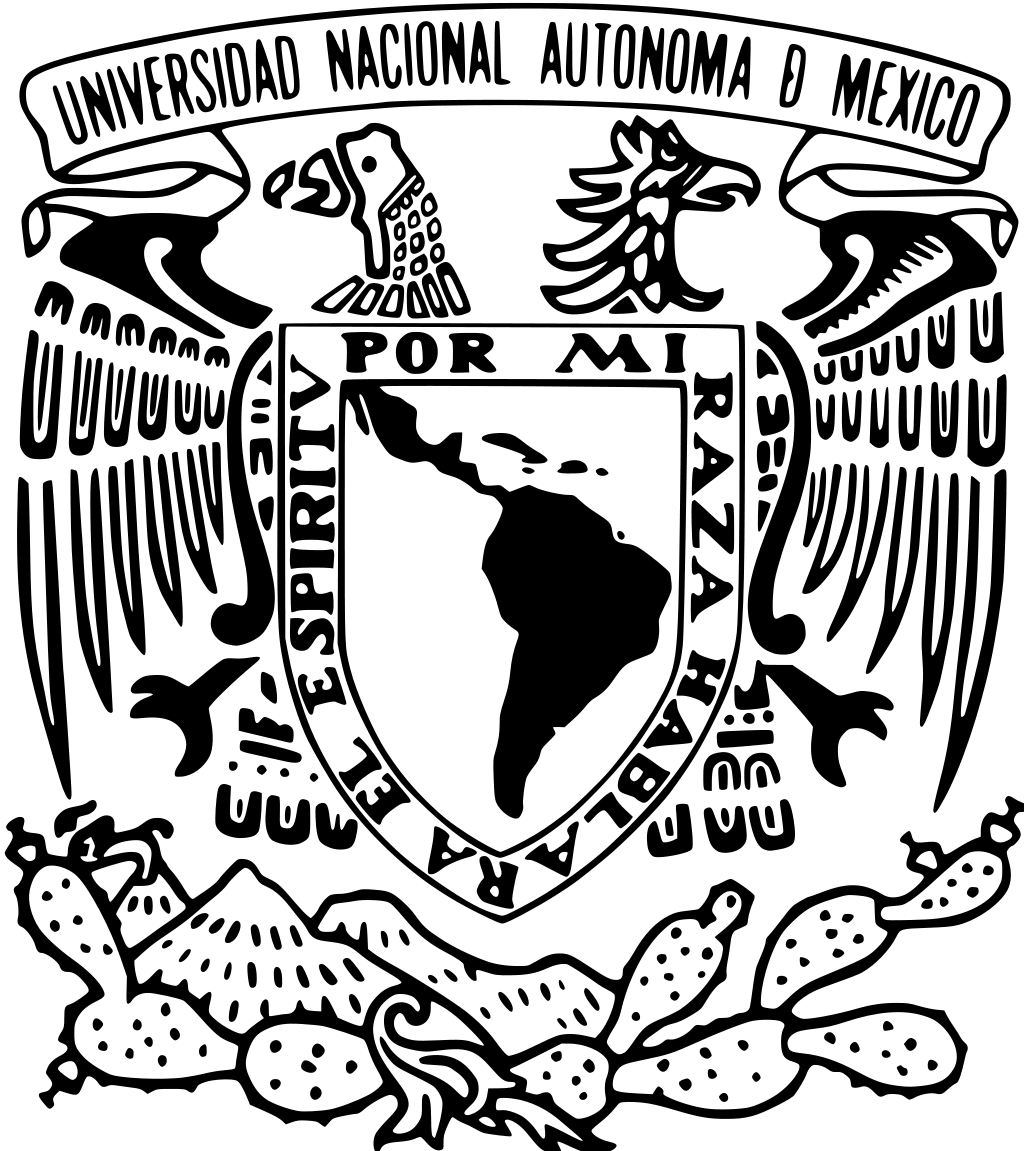
\includegraphics[width=0.25\textwidth]{../img_common/unam_logo}\vspace{0.5cm}

    {\scshape{\Large Lab. Organización y Arquitectura de Computadoras\par{}}}\vfill{}


    {\huge \textbf{\tituloTrabajo{}}}\vfill{}


    {\Large
      Alumnos
      \begin{itemize}

        \item Monsalvo Bolaños Melissa Monserrat

        \item Romero Andrade Cristian
      \end{itemize}
    }\vfill{}

      {\large Grupo: 01\par{}}\vfill{}

    {\large Profesor\\Ing.~Adrian Ulises Mercado Martinez}\vfill{}
    \vfil{}
    {\large Semestre\\\textbf{2022--1}}
    \vfill{}
    % {\large Fecha de Entrega\\\fechaEntrega}
    % \vfill{}
    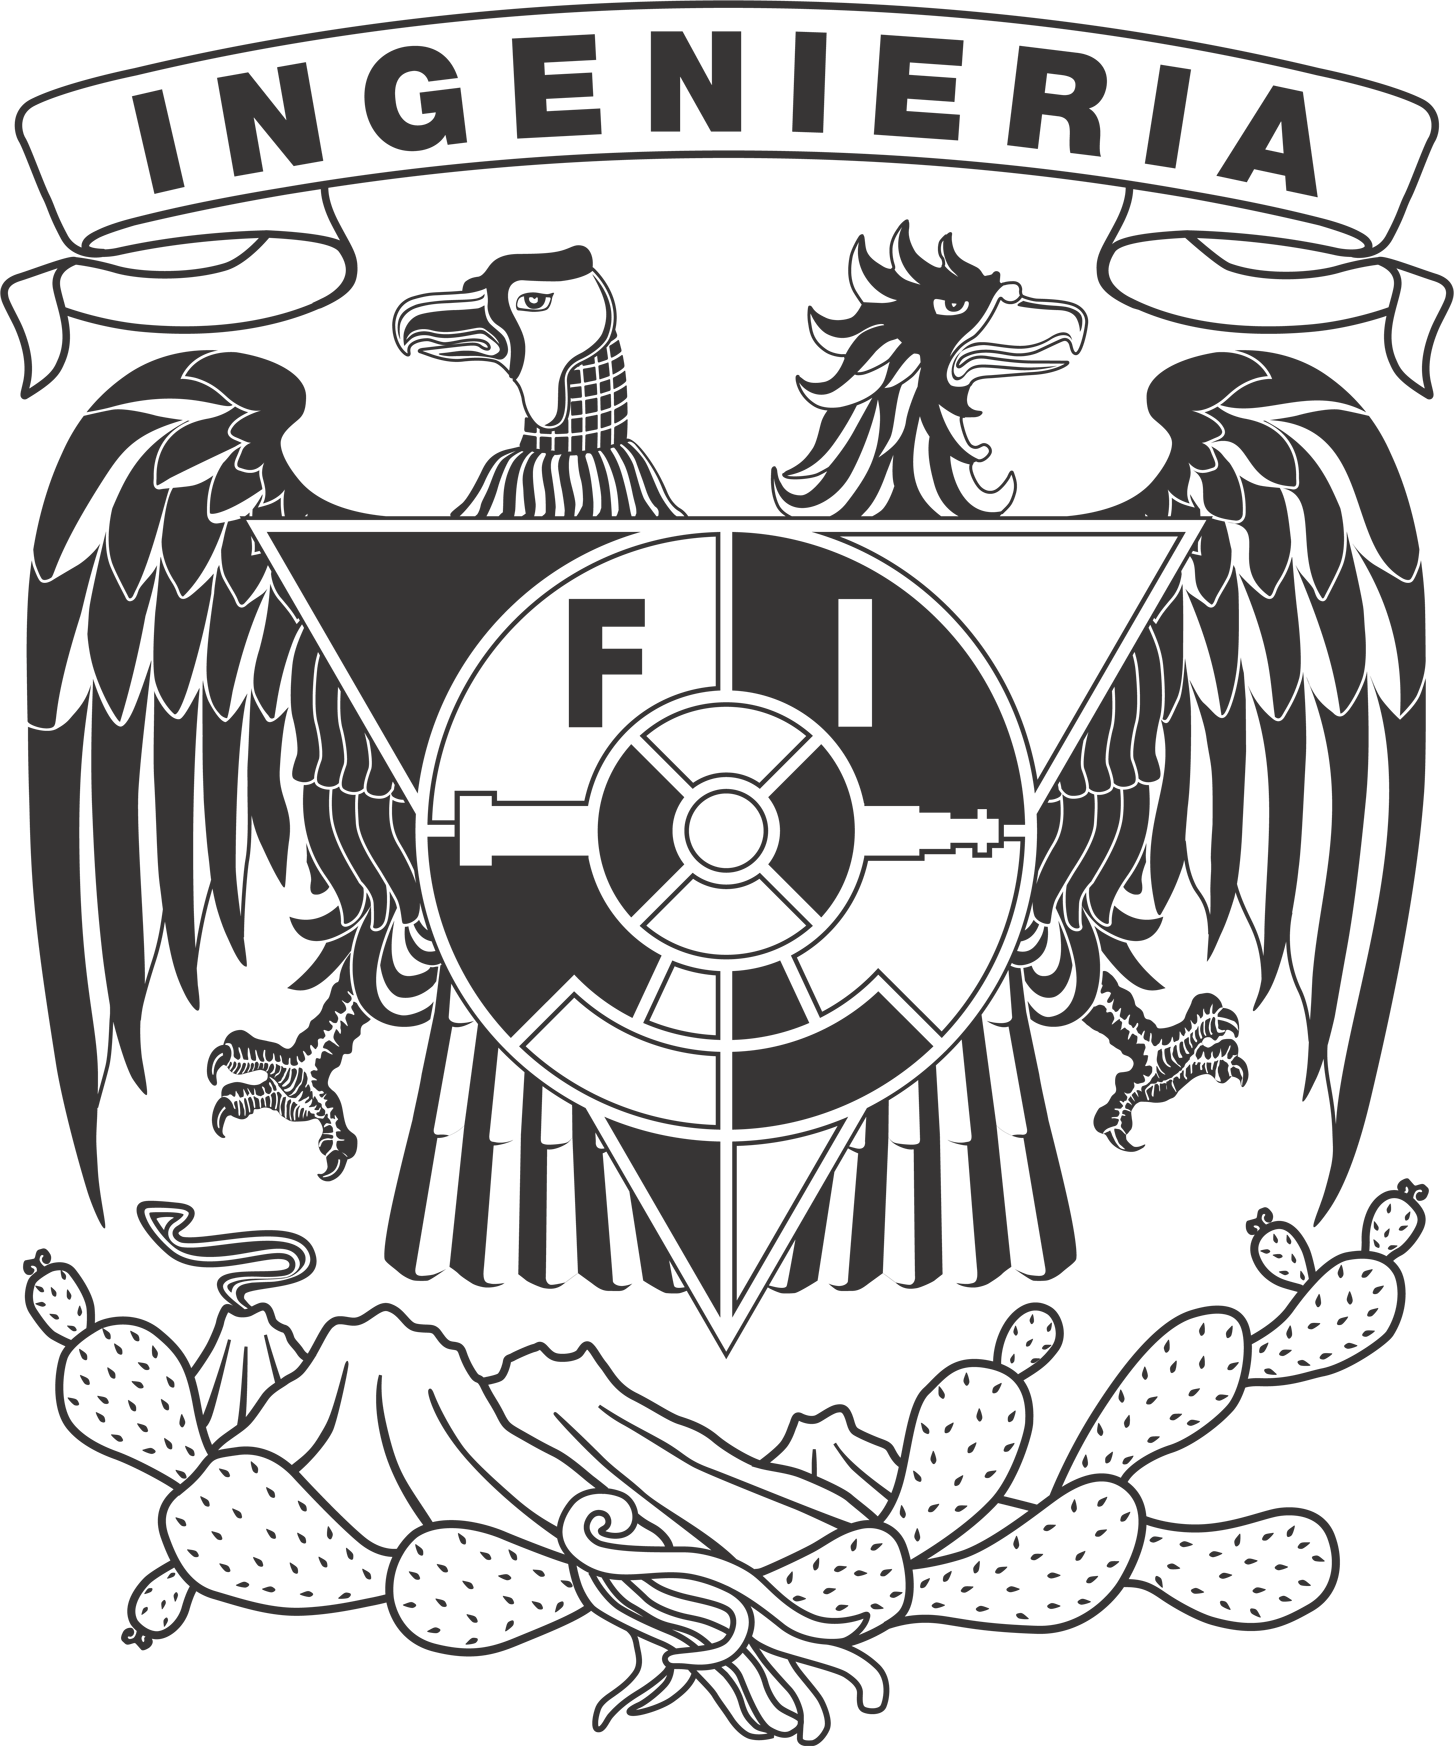
\includegraphics[width=0.1\textwidth]{../img_common/inge_logo}

\end{titlepage}

\maketitle{}
\tableofcontents{}
\section{Introducción}
\label{sec:org6bd500f}
Las máquinas de estados finitos nos sirven para realizar procesos bien
definidos en un tiempo discreto. Reciben una entrada, hacen un proceso y nos
entregan una salida.
La descripción de estas máquinas de estados finitos, en lenguaje de alto nivel,
se realiza de forma sencilla, pero en algunas ocasiones esta descripción
consume muchos recursos del dispositivo, y además el tiempo de respuesta que
dan los retardos de propagación es difícil de entender y controlar. De ahí la
necesidad de aprender a describirlos de diferentes formas en busca del diseño
más eficiente, por lo que es fundamental utilizar una arquitectura basada en el
uso de un bloque ROM de la FPGA.
\section{Objetivo}
\label{sec:org8bfa7f0}
Familiarizar al alumno en el conocimiento de construcción de máquinas de
estados usando direccionamiento de memorias con el método de
direccionamiento por trayectoria.
\section{Desarrollo}
\label{sec:orgac7043c}
El direccionamiento por trayectoria guarda el estado siguiente y las salidas de
cada estado de la carta ASM en una localidad de memoria. La porción de la
memoria que indica el estado siguiente es llamada \textbf{LIGA}, mientras que la
segunda porción de la memoria es usada para las \textbf{SALIDAS}.
\begin{figure}[htbp]
  \centering
  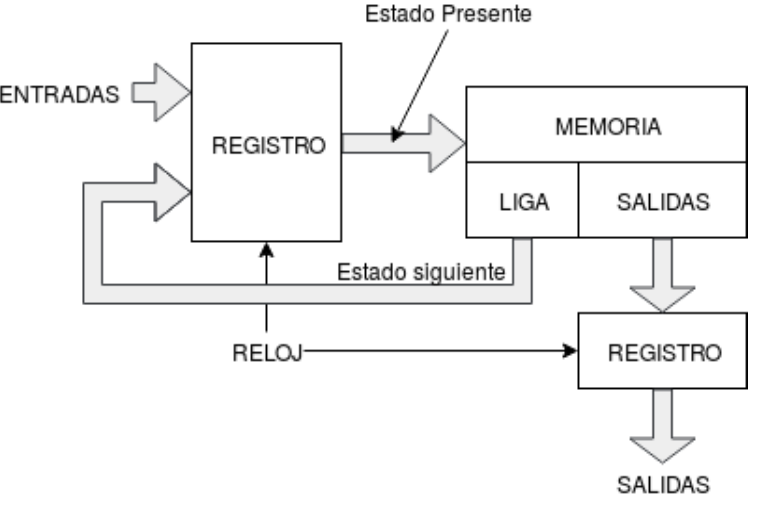
\includegraphics[width=0.3\textwidth]{./img/1.png}
  \caption{Direccionamiento por trayectoria}
\end{figure}

\begin{enumerate}
  \item Dada la carta ASM de la figura \hyperref[fig:2]{2}, encuentre el contenido de memoria
        utilizando el direccionamiento por trayectoria. Recuerde que antes de
        construir la tabla se debe asignar a cada estado de la carta ASM una
        representación binaria. Así mismo, recuerde que para cada estado es necesario
        considerar todas las posibles combinaciones de las variables de entrada, aun
        cuando algunas de ellas no se utilicen en determinado estado
        \begin{figure}[htbp]
          \centering
          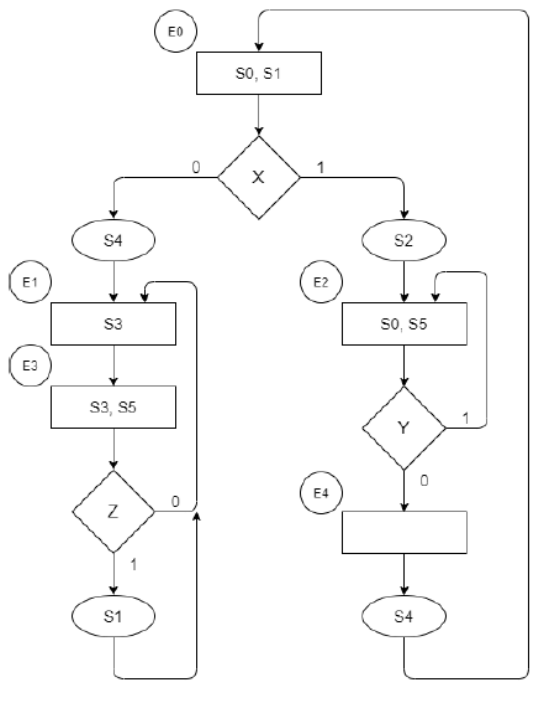
\includegraphics[width=0.3\textwidth]{./img/2.png}
          \caption{\label{fig:2}Carta ASM}
        \end{figure}

        Naturalmente asignaremos los siguientes valores binarios a la entradas:
        \begin{center}
          \centering{}
          \begin{itemize}
            \item E0 = 000
            \item E1 = 001
            \item E2 = 010
            \item E3 = 011
            \item E4 = 100
          \end{itemize}
        \end{center}
        \begin{center}
          \centering
          \captionof{table}{Contenido de la memoria}
          \begin{longtable}{|ccc|ccccccccccccccccccc|}
\hline
\rowcolor[HTML]{CC4125}
\multicolumn{3}{|c|}{\cellcolor[HTML]{CC4125}{\color[HTML]{FFFFFF} \textbf{Dirección de memoria}}} & \multicolumn{19}{c|}{\cellcolor[HTML]{CC4125}Contenido de la memoria} \\ \hline
\rowcolor[HTML]{E06666}
\multicolumn{3}{|c|}{\cellcolor[HTML]{E06666}Estado Presente} & \multicolumn{3}{c|}{\cellcolor[HTML]{E06666}} & \multicolumn{3}{c|}{\cellcolor[HTML]{E06666}} & \multicolumn{3}{c|}{\cellcolor[HTML]{E06666}} & \multicolumn{5}{c|}{\cellcolor[HTML]{E06666}Salidas Falsas} & \multicolumn{5}{c|}{\cellcolor[HTML]{E06666}Salidas Verdaderas} \\ \cline{1-3} \cline{13-22}
\rowcolor[HTML]{F6B26B}
\multicolumn{1}{|c|}{\cellcolor[HTML]{F6B26B}Q2} & \multicolumn{1}{c|}{\cellcolor[HTML]{F6B26B}Q1} & Q0 & \multicolumn{3}{c|}{\multirow{-2}{*}{\cellcolor[HTML]{E06666}Prueba}} & \multicolumn{3}{c|}{\multirow{-2}{*}{\cellcolor[HTML]{E06666}Liga Falsa}} & \multicolumn{3}{c|}{\multirow{-2}{*}{\cellcolor[HTML]{E06666}Liga Verdadera}} & \multicolumn{1}{c|}{\cellcolor[HTML]{F6B26B}S5} & \multicolumn{1}{c|}{\cellcolor[HTML]{F6B26B}S3} & \multicolumn{1}{c|}{\cellcolor[HTML]{F6B26B}S2} & \multicolumn{1}{c|}{\cellcolor[HTML]{F6B26B}S1} & \multicolumn{1}{c|}{\cellcolor[HTML]{F6B26B}S0} & \multicolumn{1}{c|}{\cellcolor[HTML]{F6B26B}S5} & \multicolumn{1}{c|}{\cellcolor[HTML]{F6B26B}S3} & \multicolumn{1}{c|}{\cellcolor[HTML]{F6B26B}S2} & \multicolumn{1}{c|}{\cellcolor[HTML]{F6B26B}S1} & S0 \\ \hline
\rowcolor[HTML]{FFE599}
\multicolumn{1}{|c|}{\cellcolor[HTML]{FFE599}0} & \multicolumn{1}{c|}{\cellcolor[HTML]{FFE599}0} & 0 & \multicolumn{1}{c|}{\cellcolor[HTML]{FFE599}1} & \multicolumn{1}{c|}{\cellcolor[HTML]{FFE599}0} & \multicolumn{1}{c|}{\cellcolor[HTML]{FFE599}0} & \multicolumn{1}{c|}{\cellcolor[HTML]{FFE599}0} & \multicolumn{1}{c|}{\cellcolor[HTML]{FFE599}0} & \multicolumn{1}{c|}{\cellcolor[HTML]{FFE599}1} & \multicolumn{1}{c|}{\cellcolor[HTML]{FFE599}0} & \multicolumn{1}{c|}{\cellcolor[HTML]{FFE599}0} & \multicolumn{1}{c|}{\cellcolor[HTML]{FFE599}1} & \multicolumn{1}{c|}{\cellcolor[HTML]{FFE599}0} & \multicolumn{1}{c|}{\cellcolor[HTML]{FFE599}0} & \multicolumn{1}{c|}{\cellcolor[HTML]{FFE599}0} & \multicolumn{1}{c|}{\cellcolor[HTML]{FFE599}0} & \multicolumn{1}{c|}{\cellcolor[HTML]{FFE599}0} & \multicolumn{1}{c|}{\cellcolor[HTML]{FFE599}0} & \multicolumn{1}{c|}{\cellcolor[HTML]{FFE599}0} & \multicolumn{1}{c|}{\cellcolor[HTML]{FFE599}0} & \multicolumn{1}{c|}{\cellcolor[HTML]{FFE599}0} & 0 \\ \hline
\rowcolor[HTML]{B6D7A8}
\multicolumn{1}{|c|}{\cellcolor[HTML]{B6D7A8}0} & \multicolumn{1}{c|}{\cellcolor[HTML]{B6D7A8}0} & 1 & \multicolumn{1}{c|}{\cellcolor[HTML]{B6D7A8}0} & \multicolumn{1}{c|}{\cellcolor[HTML]{B6D7A8}1} & \multicolumn{1}{c|}{\cellcolor[HTML]{B6D7A8}0} & \multicolumn{1}{c|}{\cellcolor[HTML]{B6D7A8}0} & \multicolumn{1}{c|}{\cellcolor[HTML]{B6D7A8}1} & \multicolumn{1}{c|}{\cellcolor[HTML]{B6D7A8}0} & \multicolumn{1}{c|}{\cellcolor[HTML]{B6D7A8}1} & \multicolumn{1}{c|}{\cellcolor[HTML]{B6D7A8}0} & \multicolumn{1}{c|}{\cellcolor[HTML]{B6D7A8}0} & \multicolumn{1}{c|}{\cellcolor[HTML]{B6D7A8}0} & \multicolumn{1}{c|}{\cellcolor[HTML]{B6D7A8}0} & \multicolumn{1}{c|}{\cellcolor[HTML]{B6D7A8}0} & \multicolumn{1}{c|}{\cellcolor[HTML]{B6D7A8}1} & \multicolumn{1}{c|}{\cellcolor[HTML]{B6D7A8}0} & \multicolumn{1}{c|}{\cellcolor[HTML]{B6D7A8}0} & \multicolumn{1}{c|}{\cellcolor[HTML]{B6D7A8}0} & \multicolumn{1}{c|}{\cellcolor[HTML]{B6D7A8}0} & \multicolumn{1}{c|}{\cellcolor[HTML]{B6D7A8}1} & 0 \\ \hline
\rowcolor[HTML]{A2C4C9}
\multicolumn{1}{|c|}{\cellcolor[HTML]{A2C4C9}0} & \multicolumn{1}{c|}{\cellcolor[HTML]{A2C4C9}1} & 0 & \multicolumn{1}{c|}{\cellcolor[HTML]{A2C4C9}1} & \multicolumn{1}{c|}{\cellcolor[HTML]{A2C4C9}0} & \multicolumn{1}{c|}{\cellcolor[HTML]{A2C4C9}0} & \multicolumn{1}{c|}{\cellcolor[HTML]{A2C4C9}0} & \multicolumn{1}{c|}{\cellcolor[HTML]{A2C4C9}1} & \multicolumn{1}{c|}{\cellcolor[HTML]{A2C4C9}1} & \multicolumn{1}{c|}{\cellcolor[HTML]{A2C4C9}0} & \multicolumn{1}{c|}{\cellcolor[HTML]{A2C4C9}1} & \multicolumn{1}{c|}{\cellcolor[HTML]{A2C4C9}1} & \multicolumn{1}{c|}{\cellcolor[HTML]{A2C4C9}0} & \multicolumn{1}{c|}{\cellcolor[HTML]{A2C4C9}0} & \multicolumn{1}{c|}{\cellcolor[HTML]{A2C4C9}0} & \multicolumn{1}{c|}{\cellcolor[HTML]{A2C4C9}0} & \multicolumn{1}{c|}{\cellcolor[HTML]{A2C4C9}0} & \multicolumn{1}{c|}{\cellcolor[HTML]{A2C4C9}0} & \multicolumn{1}{c|}{\cellcolor[HTML]{A2C4C9}0} & \multicolumn{1}{c|}{\cellcolor[HTML]{A2C4C9}0} & \multicolumn{1}{c|}{\cellcolor[HTML]{A2C4C9}0} & 0 \\ \hline
\rowcolor[HTML]{A4C2F4}
\multicolumn{1}{|c|}{\cellcolor[HTML]{A4C2F4}0} & \multicolumn{1}{c|}{\cellcolor[HTML]{A4C2F4}1} & 1 & \multicolumn{1}{c|}{\cellcolor[HTML]{A4C2F4}0} & \multicolumn{1}{c|}{\cellcolor[HTML]{A4C2F4}0} & \multicolumn{1}{c|}{\cellcolor[HTML]{A4C2F4}0} & \multicolumn{1}{c|}{\cellcolor[HTML]{A4C2F4}1} & \multicolumn{1}{c|}{\cellcolor[HTML]{A4C2F4}0} & \multicolumn{1}{c|}{\cellcolor[HTML]{A4C2F4}1} & \multicolumn{1}{c|}{\cellcolor[HTML]{A4C2F4}1} & \multicolumn{1}{c|}{\cellcolor[HTML]{A4C2F4}1} & \multicolumn{1}{c|}{\cellcolor[HTML]{A4C2F4}0} & \multicolumn{1}{c|}{\cellcolor[HTML]{A4C2F4}0} & \multicolumn{1}{c|}{\cellcolor[HTML]{A4C2F4}1} & \multicolumn{1}{c|}{\cellcolor[HTML]{A4C2F4}0} & \multicolumn{1}{c|}{\cellcolor[HTML]{A4C2F4}0} & \multicolumn{1}{c|}{\cellcolor[HTML]{A4C2F4}0} & \multicolumn{1}{c|}{\cellcolor[HTML]{A4C2F4}0} & \multicolumn{1}{c|}{\cellcolor[HTML]{A4C2F4}1} & \multicolumn{1}{c|}{\cellcolor[HTML]{A4C2F4}0} & \multicolumn{1}{c|}{\cellcolor[HTML]{A4C2F4}0} & 0 \\ \hline
\rowcolor[HTML]{9FC5E8}
\multicolumn{1}{|c|}{\cellcolor[HTML]{9FC5E8}1} & \multicolumn{1}{c|}{\cellcolor[HTML]{9FC5E8}0} & 0 & \multicolumn{1}{c|}{\cellcolor[HTML]{9FC5E8}0} & \multicolumn{1}{c|}{\cellcolor[HTML]{9FC5E8}1} & \multicolumn{1}{c|}{\cellcolor[HTML]{9FC5E8}1} & \multicolumn{1}{c|}{\cellcolor[HTML]{9FC5E8}0} & \multicolumn{1}{c|}{\cellcolor[HTML]{9FC5E8}0} & \multicolumn{1}{c|}{\cellcolor[HTML]{9FC5E8}1} & \multicolumn{1}{c|}{\cellcolor[HTML]{9FC5E8}0} & \multicolumn{1}{c|}{\cellcolor[HTML]{9FC5E8}1} & \multicolumn{1}{c|}{\cellcolor[HTML]{9FC5E8}0} & \multicolumn{1}{c|}{\cellcolor[HTML]{9FC5E8}1} & \multicolumn{1}{c|}{\cellcolor[HTML]{9FC5E8}0} & \multicolumn{1}{c|}{\cellcolor[HTML]{9FC5E8}0} & \multicolumn{1}{c|}{\cellcolor[HTML]{9FC5E8}0} & \multicolumn{1}{c|}{\cellcolor[HTML]{9FC5E8}0} & \multicolumn{1}{c|}{\cellcolor[HTML]{9FC5E8}1} & \multicolumn{1}{c|}{\cellcolor[HTML]{9FC5E8}0} & \multicolumn{1}{c|}{\cellcolor[HTML]{9FC5E8}0} & \multicolumn{1}{c|}{\cellcolor[HTML]{9FC5E8}0} & 0 \\ \hline
\rowcolor[HTML]{B4A7D6}
\multicolumn{1}{|c|}{\cellcolor[HTML]{B4A7D6}1} & \multicolumn{1}{c|}{\cellcolor[HTML]{B4A7D6}0} & 1 & \multicolumn{1}{c|}{\cellcolor[HTML]{B4A7D6}1} & \multicolumn{1}{c|}{\cellcolor[HTML]{B4A7D6}0} & \multicolumn{1}{c|}{\cellcolor[HTML]{B4A7D6}0} & \multicolumn{1}{c|}{\cellcolor[HTML]{B4A7D6}0} & \multicolumn{1}{c|}{\cellcolor[HTML]{B4A7D6}1} & \multicolumn{1}{c|}{\cellcolor[HTML]{B4A7D6}1} & \multicolumn{1}{c|}{\cellcolor[HTML]{B4A7D6}0} & \multicolumn{1}{c|}{\cellcolor[HTML]{B4A7D6}1} & \multicolumn{1}{c|}{\cellcolor[HTML]{B4A7D6}1} & \multicolumn{1}{c|}{\cellcolor[HTML]{B4A7D6}0} & \multicolumn{1}{c|}{\cellcolor[HTML]{B4A7D6}0} & \multicolumn{1}{c|}{\cellcolor[HTML]{B4A7D6}0} & \multicolumn{1}{c|}{\cellcolor[HTML]{B4A7D6}0} & \multicolumn{1}{c|}{\cellcolor[HTML]{B4A7D6}0} & \multicolumn{1}{c|}{\cellcolor[HTML]{B4A7D6}0} & \multicolumn{1}{c|}{\cellcolor[HTML]{B4A7D6}0} & \multicolumn{1}{c|}{\cellcolor[HTML]{B4A7D6}0} & \multicolumn{1}{c|}{\cellcolor[HTML]{B4A7D6}0} & 0 \\ \hline
\rowcolor[HTML]{D5A6BD}
\multicolumn{1}{|c|}{\cellcolor[HTML]{D5A6BD}1} & \multicolumn{1}{c|}{\cellcolor[HTML]{D5A6BD}1} & 0 & \multicolumn{1}{c|}{\cellcolor[HTML]{D5A6BD}0} & \multicolumn{1}{c|}{\cellcolor[HTML]{D5A6BD}0} & \multicolumn{1}{c|}{\cellcolor[HTML]{D5A6BD}1} & \multicolumn{1}{c|}{\cellcolor[HTML]{D5A6BD}1} & \multicolumn{1}{c|}{\cellcolor[HTML]{D5A6BD}0} & \multicolumn{1}{c|}{\cellcolor[HTML]{D5A6BD}1} & \multicolumn{1}{c|}{\cellcolor[HTML]{D5A6BD}0} & \multicolumn{1}{c|}{\cellcolor[HTML]{D5A6BD}1} & \multicolumn{1}{c|}{\cellcolor[HTML]{D5A6BD}0} & \multicolumn{1}{c|}{\cellcolor[HTML]{D5A6BD}0} & \multicolumn{1}{c|}{\cellcolor[HTML]{D5A6BD}0} & \multicolumn{1}{c|}{\cellcolor[HTML]{D5A6BD}0} & \multicolumn{1}{c|}{\cellcolor[HTML]{D5A6BD}1} & \multicolumn{1}{c|}{\cellcolor[HTML]{D5A6BD}0} & \multicolumn{1}{c|}{\cellcolor[HTML]{D5A6BD}1} & \multicolumn{1}{c|}{\cellcolor[HTML]{D5A6BD}0} & \multicolumn{1}{c|}{\cellcolor[HTML]{D5A6BD}0} & \multicolumn{1}{c|}{\cellcolor[HTML]{D5A6BD}1} & 0 \\ \hline
\end{longtable}

        \end{center}
  \item Una vez que haya obtenido el contenido de memoria, implemente el
        direccionamiento por trayectoria utilizando el software de desarrollo
        Quartus y escriba el contenido de memoria obtenido.
        \begin{code}
          \inputminted{vhdl}{./memoria_rom.vhd}
          \caption{\texttt{memoria_rom.vhd}}
        \end{code}
        \begin{code}
          \inputminted{vhdl}{./registros_entrada.vhd}
          \caption{\texttt{registros_entrada.vhd}}
        \end{code}
        Escribimos código que se usará para pasar los registros de un bloque a otro,
        para ello creamos el separador y la salida.
        \begin{code}
          \inputminted{vhdl}{./separador.vhd}
          \caption{\texttt{separador.vhd}}
        \end{code}

        Después de que verificamos todos los archivos, creamos los símbolos, de la
        barra de herramientas seleccionamos File$\rightarrow$Create/Update$\rightarrow$Create symbols for
        current file para cada archivo vhd.

        Luego creamos un diagrama de bloques donde los conectamos y
        especificamos su salida (como se muestra en la figura \hyperref[fig:3]{3}).
        \begin{figure}[htbp]
          \centering
          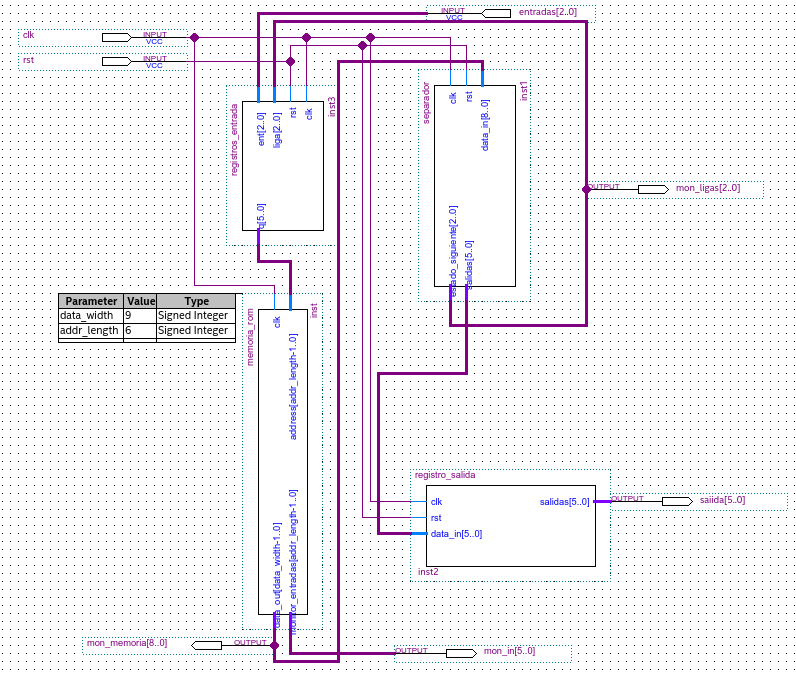
\includegraphics[width=0.9\textwidth]{./img/3.png}
          \label{fig:3}
          \caption{Diagrama de bloques de los archivos vhd}
        \end{figure}


  \item Simule su diseño para probar su funcionamiento. Recuerden que en sus
        simulaciones debe aparecer el contenido de la memoria además del
        estado presente.

        Para poder compilar el diagrama de bloques hay que seleccionar el archivo
        \texttt{*.bdf} que generamos como Top entity en las propiedades del proyecto.
        Adicionalmente se añadió unos monitores de memoria y de ligas en las salidas.
        \begin{figure}[htbp]
          \centering
          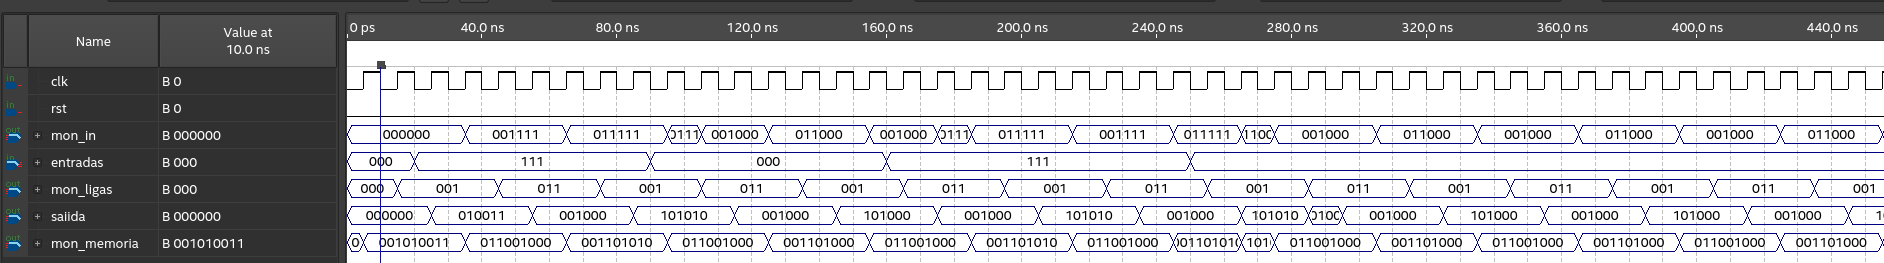
\includegraphics[width=0.9\textwidth]{./img/4.png}\label{fig:4}
          \caption{Simulación}
        \end{figure}
\end{enumerate}
\section{Conclusiones}
\label{sec:orgdab2190}

\subsection*{Monsalvo Bolaños Melissa Monserrat}\label{sec:mons-bolan-melissa}



Con el desarrollo de esta práctica pudimos describir una máquina ASM con el
lenguaje VHDL siguiendo el método de direccionamiento por trayectoria y
utilizando una memoria ROM y tres registros, uno de entrada, uno de salida y un
separador de la salida que dividía la liga de las salidas. Realizamos bloques de
cada una de las partes y a través de un diagrama esquemático realizamos las
conexiones. Además pudimos comprobar su funcionamiento a través de la
simulación.

\subsection*{Romero Andrade Cristian}
\label{sec:romero-andr-crist}



El software de quartus nos facilita la
implementación de nuestras tablas de verdad que generamos a partir de la carta
ASM, si bien se puede hacer todo con código VHDL, el uso de los diagramas de
bloques nos da “una pista” de los recursos que podremos utilizar a la hora de
crear nuestro dispositivo.

\subsection*{Conclusiones en equipo}
\label{sec:concl-en-equipo}



Con esta práctica pudimos implementar en el
lenguaje VHDL una máquina ASM y para ello utilizamos el direccionamiento por
trayectoria y con la ayuda de Quartus pudimos realizar un diagrama
esquemático de sus componentes. Para obtener las salidas correspondientes,
primero obtuvimos la tabla de verdad que consideraba las entradas X, Y y Z y la
liga.

\nocite{*}
\addcontentsline{toc}{section}{Referencias}
\printbibliography{}
\end{document}
